%\documentclass[dvipdfmx]{beamer}      % platex の場合
\documentclass{beamer}                 % lualatex の場合
\usepackage{mySld}
\usepackage{multicol}

\begin{document}
\title{基礎コンピュータ工学\\第5章 機械語プログラミング\\(パート7)}
\date{}

\begin{frame}
  \titlepage
\end{frame}

%==============================================================================
%\begin{frame}
%  \frametitle
%  \tableofcontents
%\end{frame}

\section{繰り返し}
%==============================================================================
\begin{frame}
  \frametitle{繰り返し処理(1)}
  ループの最後で条件判断する例(Javaの do ... while に似ている)\\
  \vfill
  \centerline{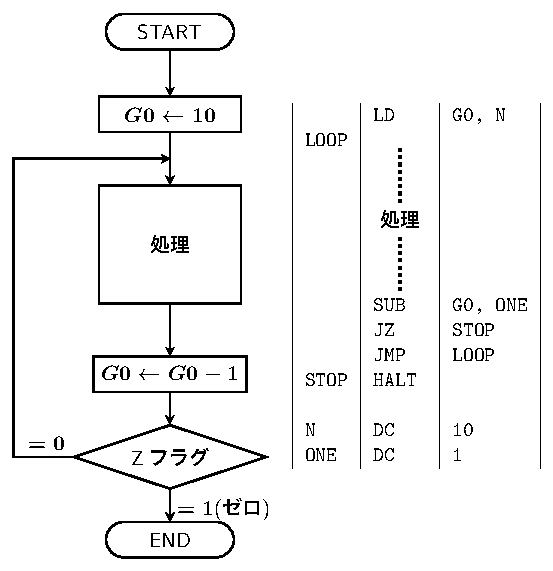
\includegraphics[scale=0.7]{../Tikz/flow2.pdf}}
  \vfill
\end{frame}

%==============================================================================
\begin{frame}
  \frametitle{繰り返し処理(2)}
  ループの最初で条件判断する例(Javaの while に似ている)
  \vfill
  \centerline{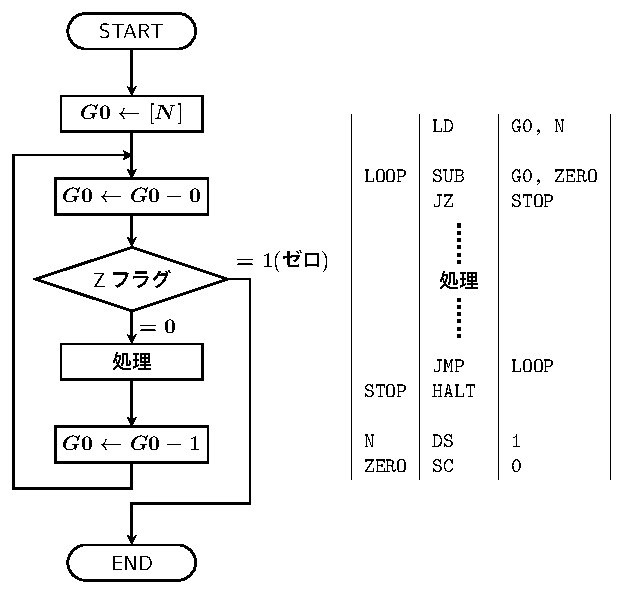
\includegraphics[scale=0.7]{../Tikz/flow2C.pdf}}
  \vfill
\end{frame}

%==============================================================================
\begin{frame}
  \frametitle{繰り返しの例}
  $1 + 2 + 3 + ... + 10$を計算する.(例題5-2)\\
  \vfill
  \begin{minipage}{0.47\columnwidth}
    \centerline{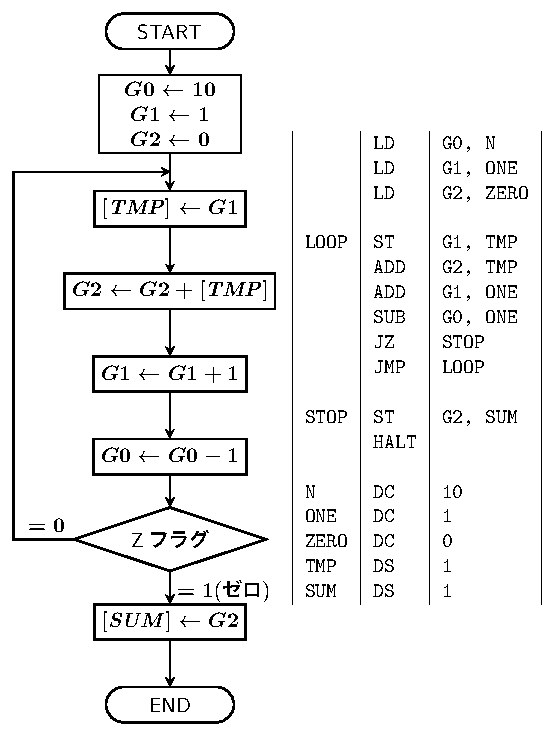
\includegraphics[scale=0.55]{../Tikz/flow3.pdf}}
  \end{minipage}
  \begin{minipage}{0.52\columnwidth}
    {\ttfamily
      G0,G1,G2,SP が使用可能.\\
      これらの役割を決める.\\
      例えば次のように割り振る.
      \begin{itemize}
      \item G0:繰り返し回数のカウンタ
      \item G1:足す数(1,2,3,...,10)
      \item G2:合計(足される数)
      \item G2 ← G2 + G1 はできない \\
        次の2ステップに分解する.
        \begin{itemize}
          \item $[TMP] ← G1$
          \item $G2 ←G2 + [TMP]$
        \end{itemize}
      \end{itemize}
    }
  \end{minipage}
  \vfill
\end{frame}

%==============================================================================
\begin{frame}
  \frametitle{まとめ}
  \emph{学んだこと}
  \begin{itemize}
  \item 条件判断の追加の演習
  \item 繰り返し処理
    \begin{itemize}
    \item 最後で条件判断(繰り返し処理1)
    \item 最初で条件判断(繰り返し処理2)
    \end{itemize}
  \item 繰り返しの例(例題5-2)
  \end{itemize}
  \vfill

  \emph{演習(宿題)}
  \begin{itemize}
  \item \emph{掛け算プログラム}:N番地のデータと,
    M番地のデータのかけ算を計算しL番地に格納するプログラム
  \item データはどれも符号なし整数とする.
  \item 繰り返し処理1のフローチャートを参考に作る.
  \end{itemize}
  \vfill
\end{frame}

\end{document}
